% Options for packages loaded elsewhere
\PassOptionsToPackage{unicode}{hyperref}
\PassOptionsToPackage{hyphens}{url}
\PassOptionsToPackage{dvipsnames,svgnames,x11names}{xcolor}
%
\documentclass[
]{scrartcl}

\usepackage{amsmath,amssymb}
\usepackage{iftex}
\ifPDFTeX
  \usepackage[T1]{fontenc}
  \usepackage[utf8]{inputenc}
  \usepackage{textcomp} % provide euro and other symbols
\else % if luatex or xetex
  \usepackage{unicode-math}
  \defaultfontfeatures{Scale=MatchLowercase}
  \defaultfontfeatures[\rmfamily]{Ligatures=TeX,Scale=1}
\fi
\usepackage{lmodern}
\ifPDFTeX\else  
    % xetex/luatex font selection
\fi
% Use upquote if available, for straight quotes in verbatim environments
\IfFileExists{upquote.sty}{\usepackage{upquote}}{}
\IfFileExists{microtype.sty}{% use microtype if available
  \usepackage[]{microtype}
  \UseMicrotypeSet[protrusion]{basicmath} % disable protrusion for tt fonts
}{}
\makeatletter
\@ifundefined{KOMAClassName}{% if non-KOMA class
  \IfFileExists{parskip.sty}{%
    \usepackage{parskip}
  }{% else
    \setlength{\parindent}{0pt}
    \setlength{\parskip}{6pt plus 2pt minus 1pt}}
}{% if KOMA class
  \KOMAoptions{parskip=half}}
\makeatother
\usepackage{xcolor}
\setlength{\emergencystretch}{3em} % prevent overfull lines
\setcounter{secnumdepth}{-\maxdimen} % remove section numbering
% Make \paragraph and \subparagraph free-standing
\ifx\paragraph\undefined\else
  \let\oldparagraph\paragraph
  \renewcommand{\paragraph}[1]{\oldparagraph{#1}\mbox{}}
\fi
\ifx\subparagraph\undefined\else
  \let\oldsubparagraph\subparagraph
  \renewcommand{\subparagraph}[1]{\oldsubparagraph{#1}\mbox{}}
\fi

\usepackage{color}
\usepackage{fancyvrb}
\newcommand{\VerbBar}{|}
\newcommand{\VERB}{\Verb[commandchars=\\\{\}]}
\DefineVerbatimEnvironment{Highlighting}{Verbatim}{commandchars=\\\{\}}
% Add ',fontsize=\small' for more characters per line
\usepackage{framed}
\definecolor{shadecolor}{RGB}{241,243,245}
\newenvironment{Shaded}{\begin{snugshade}}{\end{snugshade}}
\newcommand{\AlertTok}[1]{\textcolor[rgb]{0.68,0.00,0.00}{#1}}
\newcommand{\AnnotationTok}[1]{\textcolor[rgb]{0.37,0.37,0.37}{#1}}
\newcommand{\AttributeTok}[1]{\textcolor[rgb]{0.40,0.45,0.13}{#1}}
\newcommand{\BaseNTok}[1]{\textcolor[rgb]{0.68,0.00,0.00}{#1}}
\newcommand{\BuiltInTok}[1]{\textcolor[rgb]{0.00,0.23,0.31}{#1}}
\newcommand{\CharTok}[1]{\textcolor[rgb]{0.13,0.47,0.30}{#1}}
\newcommand{\CommentTok}[1]{\textcolor[rgb]{0.37,0.37,0.37}{#1}}
\newcommand{\CommentVarTok}[1]{\textcolor[rgb]{0.37,0.37,0.37}{\textit{#1}}}
\newcommand{\ConstantTok}[1]{\textcolor[rgb]{0.56,0.35,0.01}{#1}}
\newcommand{\ControlFlowTok}[1]{\textcolor[rgb]{0.00,0.23,0.31}{#1}}
\newcommand{\DataTypeTok}[1]{\textcolor[rgb]{0.68,0.00,0.00}{#1}}
\newcommand{\DecValTok}[1]{\textcolor[rgb]{0.68,0.00,0.00}{#1}}
\newcommand{\DocumentationTok}[1]{\textcolor[rgb]{0.37,0.37,0.37}{\textit{#1}}}
\newcommand{\ErrorTok}[1]{\textcolor[rgb]{0.68,0.00,0.00}{#1}}
\newcommand{\ExtensionTok}[1]{\textcolor[rgb]{0.00,0.23,0.31}{#1}}
\newcommand{\FloatTok}[1]{\textcolor[rgb]{0.68,0.00,0.00}{#1}}
\newcommand{\FunctionTok}[1]{\textcolor[rgb]{0.28,0.35,0.67}{#1}}
\newcommand{\ImportTok}[1]{\textcolor[rgb]{0.00,0.46,0.62}{#1}}
\newcommand{\InformationTok}[1]{\textcolor[rgb]{0.37,0.37,0.37}{#1}}
\newcommand{\KeywordTok}[1]{\textcolor[rgb]{0.00,0.23,0.31}{#1}}
\newcommand{\NormalTok}[1]{\textcolor[rgb]{0.00,0.23,0.31}{#1}}
\newcommand{\OperatorTok}[1]{\textcolor[rgb]{0.37,0.37,0.37}{#1}}
\newcommand{\OtherTok}[1]{\textcolor[rgb]{0.00,0.23,0.31}{#1}}
\newcommand{\PreprocessorTok}[1]{\textcolor[rgb]{0.68,0.00,0.00}{#1}}
\newcommand{\RegionMarkerTok}[1]{\textcolor[rgb]{0.00,0.23,0.31}{#1}}
\newcommand{\SpecialCharTok}[1]{\textcolor[rgb]{0.37,0.37,0.37}{#1}}
\newcommand{\SpecialStringTok}[1]{\textcolor[rgb]{0.13,0.47,0.30}{#1}}
\newcommand{\StringTok}[1]{\textcolor[rgb]{0.13,0.47,0.30}{#1}}
\newcommand{\VariableTok}[1]{\textcolor[rgb]{0.07,0.07,0.07}{#1}}
\newcommand{\VerbatimStringTok}[1]{\textcolor[rgb]{0.13,0.47,0.30}{#1}}
\newcommand{\WarningTok}[1]{\textcolor[rgb]{0.37,0.37,0.37}{\textit{#1}}}

\providecommand{\tightlist}{%
  \setlength{\itemsep}{0pt}\setlength{\parskip}{0pt}}\usepackage{longtable,booktabs,array}
\usepackage{calc} % for calculating minipage widths
% Correct order of tables after \paragraph or \subparagraph
\usepackage{etoolbox}
\makeatletter
\patchcmd\longtable{\par}{\if@noskipsec\mbox{}\fi\par}{}{}
\makeatother
% Allow footnotes in longtable head/foot
\IfFileExists{footnotehyper.sty}{\usepackage{footnotehyper}}{\usepackage{footnote}}
\makesavenoteenv{longtable}
\usepackage{graphicx}
\makeatletter
\def\maxwidth{\ifdim\Gin@nat@width>\linewidth\linewidth\else\Gin@nat@width\fi}
\def\maxheight{\ifdim\Gin@nat@height>\textheight\textheight\else\Gin@nat@height\fi}
\makeatother
% Scale images if necessary, so that they will not overflow the page
% margins by default, and it is still possible to overwrite the defaults
% using explicit options in \includegraphics[width, height, ...]{}
\setkeys{Gin}{width=\maxwidth,height=\maxheight,keepaspectratio}
% Set default figure placement to htbp
\makeatletter
\def\fps@figure{htbp}
\makeatother

\usepackage[noblocks]{authblk}
\renewcommand*{\Authsep}{, }
\renewcommand*{\Authand}{, }
\renewcommand*{\Authands}{, }
\renewcommand\Affilfont{\small}
\makeatletter
\@ifpackageloaded{caption}{}{\usepackage{caption}}
\AtBeginDocument{%
\ifdefined\contentsname
  \renewcommand*\contentsname{Table of contents}
\else
  \newcommand\contentsname{Table of contents}
\fi
\ifdefined\listfigurename
  \renewcommand*\listfigurename{List of Figures}
\else
  \newcommand\listfigurename{List of Figures}
\fi
\ifdefined\listtablename
  \renewcommand*\listtablename{List of Tables}
\else
  \newcommand\listtablename{List of Tables}
\fi
\ifdefined\figurename
  \renewcommand*\figurename{Figure}
\else
  \newcommand\figurename{Figure}
\fi
\ifdefined\tablename
  \renewcommand*\tablename{Table}
\else
  \newcommand\tablename{Table}
\fi
}
\@ifpackageloaded{float}{}{\usepackage{float}}
\floatstyle{ruled}
\@ifundefined{c@chapter}{\newfloat{codelisting}{h}{lop}}{\newfloat{codelisting}{h}{lop}[chapter]}
\floatname{codelisting}{Listing}
\newcommand*\listoflistings{\listof{codelisting}{List of Listings}}
\makeatother
\makeatletter
\makeatother
\makeatletter
\@ifpackageloaded{caption}{}{\usepackage{caption}}
\@ifpackageloaded{subcaption}{}{\usepackage{subcaption}}
\makeatother
\ifLuaTeX
  \usepackage{selnolig}  % disable illegal ligatures
\fi
\usepackage{bookmark}

\IfFileExists{xurl.sty}{\usepackage{xurl}}{} % add URL line breaks if available
\urlstyle{same} % disable monospaced font for URLs
\hypersetup{
  pdftitle={Cumulative Abnormal Returns},
  pdfauthor={Calvin J. Chiou},
  colorlinks=true,
  linkcolor={blue},
  filecolor={Maroon},
  citecolor={Blue},
  urlcolor={Blue},
  pdfcreator={LaTeX via pandoc}}

\title{Cumulative Abnormal Returns}


  \author{Calvin J. Chiou}
  
\date{2024-05-31}
\begin{document}
\maketitle

\renewcommand*\contentsname{Table of contents}
{
\hypersetup{linkcolor=}
\setcounter{tocdepth}{1}
\tableofcontents
}
\section{Introduction}\label{introduction}

In this document, we will extend the analysis from estimating the beta
coefficient to measuring cumulative abnormal returns (CAR). CAR is used
in event studies to assess the impact of a specific event on a stock's
price. We will first estimate the market model, calculate abnormal
returns, and then compute the cumulative abnormal returns.

\subsection{Setup}\label{setup}

First, we need to install and load the required packages. Ensure you
have `tidyquant`, `dplyr`, `broom`, `knitr`, `ggplot2`, and `lubridate`
installed.

\begin{Shaded}
\begin{Highlighting}[]
\CommentTok{\# Install the necessary packages if not already installed}
\ControlFlowTok{if}\NormalTok{ (}\SpecialCharTok{!}\FunctionTok{require}\NormalTok{(tidyquant)) }\FunctionTok{install.packages}\NormalTok{(}\StringTok{"tidyquant"}\NormalTok{)}
\ControlFlowTok{if}\NormalTok{ (}\SpecialCharTok{!}\FunctionTok{require}\NormalTok{(dplyr)) }\FunctionTok{install.packages}\NormalTok{(}\StringTok{"dplyr"}\NormalTok{)}
\ControlFlowTok{if}\NormalTok{ (}\SpecialCharTok{!}\FunctionTok{require}\NormalTok{(tidyr)) }\FunctionTok{install.packages}\NormalTok{(}\StringTok{"tidyr"}\NormalTok{)}
\ControlFlowTok{if}\NormalTok{ (}\SpecialCharTok{!}\FunctionTok{require}\NormalTok{(broom)) }\FunctionTok{install.packages}\NormalTok{(}\StringTok{"broom"}\NormalTok{)}
\ControlFlowTok{if}\NormalTok{ (}\SpecialCharTok{!}\FunctionTok{require}\NormalTok{(knitr)) }\FunctionTok{install.packages}\NormalTok{(}\StringTok{"knitr"}\NormalTok{)}
\ControlFlowTok{if}\NormalTok{ (}\SpecialCharTok{!}\FunctionTok{require}\NormalTok{(ggplot2)) }\FunctionTok{install.packages}\NormalTok{(}\StringTok{"ggplot2"}\NormalTok{)}
\ControlFlowTok{if}\NormalTok{ (}\SpecialCharTok{!}\FunctionTok{require}\NormalTok{(lubridate)) }\FunctionTok{install.packages}\NormalTok{(}\StringTok{"lubridate"}\NormalTok{)}
\CommentTok{\# Load the packages}
\FunctionTok{library}\NormalTok{(tidyquant)}
\FunctionTok{library}\NormalTok{(dplyr)}
\FunctionTok{library}\NormalTok{(tidyr)}
\FunctionTok{library}\NormalTok{(broom)}
\FunctionTok{library}\NormalTok{(knitr)}
\FunctionTok{library}\NormalTok{(ggplot2)}
\FunctionTok{library}\NormalTok{(lubridate)}
\end{Highlighting}
\end{Shaded}

\section{Data Collection and
Manipulation}\label{data-collection-and-manipulation}

\subsection{\texorpdfstring{\textbf{Data
Download}}{Data Download}}\label{data-download}

We will download stock prices for a chosen stock (e.g., Apple Inc.,
ticker: AAPL) and a market index (e.g., S\&P 500, ticker: \^{}GSPC) from
Yahoo Finance during the estimation window 2020-2022. You can find any
corresponding tickers that you would like to explore from its
\href{https://finance.yahoo.com/}{website}.

\begin{Shaded}
\begin{Highlighting}[]
\CommentTok{\# Define the tickers for the stock and the market index}
\NormalTok{stock\_ticker }\OtherTok{\textless{}{-}} \StringTok{"AAPL"}
\NormalTok{market\_ticker }\OtherTok{\textless{}{-}} \StringTok{"\^{}GSPC"}

\CommentTok{\# Set the time period for the data}
\NormalTok{start\_date }\OtherTok{\textless{}{-}} \StringTok{"2020{-}01{-}01"}
\NormalTok{end\_date }\OtherTok{\textless{}{-}} \StringTok{"2023{-}01{-}01"}

\CommentTok{\# Download stock and market data}
\NormalTok{stock\_data }\OtherTok{\textless{}{-}} \FunctionTok{tq\_get}\NormalTok{(stock\_ticker, }\AttributeTok{from =}\NormalTok{ start\_date, }\AttributeTok{to =}\NormalTok{ end\_date)}
\NormalTok{market\_data }\OtherTok{\textless{}{-}} \FunctionTok{tq\_get}\NormalTok{(market\_ticker, }\AttributeTok{from =}\NormalTok{ start\_date, }\AttributeTok{to =}\NormalTok{ end\_date)}
\end{Highlighting}
\end{Shaded}

\subsection{\texorpdfstring{\textbf{Preview
Data}}{Preview Data}}\label{preview-data}

Let's take a look at the first few rows of the stock data in a pretty
format.

\begin{Shaded}
\begin{Highlighting}[]
\CommentTok{\# Print the head of the stock data in a pretty format}
\FunctionTok{kable}\NormalTok{(}\FunctionTok{head}\NormalTok{(stock\_data), }\AttributeTok{caption =} \StringTok{"Stock Data: Apple Inc. (AAPL)"}\NormalTok{)}
\end{Highlighting}
\end{Shaded}

\begin{longtable}[]{@{}
  >{\raggedright\arraybackslash}p{(\columnwidth - 14\tabcolsep) * \real{0.1014}}
  >{\raggedright\arraybackslash}p{(\columnwidth - 14\tabcolsep) * \real{0.1594}}
  >{\raggedleft\arraybackslash}p{(\columnwidth - 14\tabcolsep) * \real{0.1159}}
  >{\raggedleft\arraybackslash}p{(\columnwidth - 14\tabcolsep) * \real{0.1159}}
  >{\raggedleft\arraybackslash}p{(\columnwidth - 14\tabcolsep) * \real{0.1159}}
  >{\raggedleft\arraybackslash}p{(\columnwidth - 14\tabcolsep) * \real{0.1159}}
  >{\raggedleft\arraybackslash}p{(\columnwidth - 14\tabcolsep) * \real{0.1449}}
  >{\raggedleft\arraybackslash}p{(\columnwidth - 14\tabcolsep) * \real{0.1304}}@{}}
\caption{Stock Data: Apple Inc.~(AAPL)}\tabularnewline
\toprule\noalign{}
\begin{minipage}[b]{\linewidth}\raggedright
symbol
\end{minipage} & \begin{minipage}[b]{\linewidth}\raggedright
date
\end{minipage} & \begin{minipage}[b]{\linewidth}\raggedleft
open
\end{minipage} & \begin{minipage}[b]{\linewidth}\raggedleft
high
\end{minipage} & \begin{minipage}[b]{\linewidth}\raggedleft
low
\end{minipage} & \begin{minipage}[b]{\linewidth}\raggedleft
close
\end{minipage} & \begin{minipage}[b]{\linewidth}\raggedleft
volume
\end{minipage} & \begin{minipage}[b]{\linewidth}\raggedleft
adjusted
\end{minipage} \\
\midrule\noalign{}
\endfirsthead
\toprule\noalign{}
\begin{minipage}[b]{\linewidth}\raggedright
symbol
\end{minipage} & \begin{minipage}[b]{\linewidth}\raggedright
date
\end{minipage} & \begin{minipage}[b]{\linewidth}\raggedleft
open
\end{minipage} & \begin{minipage}[b]{\linewidth}\raggedleft
high
\end{minipage} & \begin{minipage}[b]{\linewidth}\raggedleft
low
\end{minipage} & \begin{minipage}[b]{\linewidth}\raggedleft
close
\end{minipage} & \begin{minipage}[b]{\linewidth}\raggedleft
volume
\end{minipage} & \begin{minipage}[b]{\linewidth}\raggedleft
adjusted
\end{minipage} \\
\midrule\noalign{}
\endhead
\bottomrule\noalign{}
\endlastfoot
AAPL & 2020-01-02 & 74.0600 & 75.1500 & 73.7975 & 75.0875 & 135480400 &
72.96047 \\
AAPL & 2020-01-03 & 74.2875 & 75.1450 & 74.1250 & 74.3575 & 146322800 &
72.25113 \\
AAPL & 2020-01-06 & 73.4475 & 74.9900 & 73.1875 & 74.9500 & 118387200 &
72.82687 \\
AAPL & 2020-01-07 & 74.9600 & 75.2250 & 74.3700 & 74.5975 & 108872000 &
72.48435 \\
AAPL & 2020-01-08 & 74.2900 & 76.1100 & 74.2900 & 75.7975 & 132079200 &
73.65034 \\
AAPL & 2020-01-09 & 76.8100 & 77.6075 & 76.5500 & 77.4075 & 170108400 &
75.21473 \\
\end{longtable}

\subsection{Data Preparation}\label{data-preparation}

Next, we will prepare the data by calculating daily returns for both the
stock and the market index.

\begin{Shaded}
\begin{Highlighting}[]
\CommentTok{\# Calculate daily returns for the stock and the market}
\NormalTok{stock\_returns }\OtherTok{\textless{}{-}}\NormalTok{ stock\_data }\SpecialCharTok{\%\textgreater{}\%}
  \FunctionTok{tq\_transmute}\NormalTok{(}\AttributeTok{select =}\NormalTok{ adjusted, }
               \AttributeTok{mutate\_fun =}\NormalTok{ periodReturn, }
               \AttributeTok{period =} \StringTok{"daily"}\NormalTok{, }
               \AttributeTok{col\_rename =} \StringTok{"stock\_return"}\NormalTok{)}

\NormalTok{market\_returns }\OtherTok{\textless{}{-}}\NormalTok{ market\_data }\SpecialCharTok{\%\textgreater{}\%}
  \FunctionTok{tq\_transmute}\NormalTok{(}\AttributeTok{select =}\NormalTok{ adjusted, }
               \AttributeTok{mutate\_fun =}\NormalTok{ periodReturn, }
               \AttributeTok{period =} \StringTok{"daily"}\NormalTok{, }
               \AttributeTok{col\_rename =} \StringTok{"market\_return"}\NormalTok{)}

\CommentTok{\# Combine the returns data into one data frame}
\NormalTok{returns\_data }\OtherTok{\textless{}{-}} \FunctionTok{left\_join}\NormalTok{(stock\_returns, }
\NormalTok{                          market\_returns, }
                          \AttributeTok{by =} \StringTok{"date"}\NormalTok{) }\SpecialCharTok{\%\textgreater{}\%}
  \FunctionTok{na.omit}\NormalTok{()}
\end{Highlighting}
\end{Shaded}

\section{Estimating the Market Model}\label{estimating-the-market-model}

The market model is a statistical model that describes the relationship
between the returns of a stock and the returns of the overall market. We
will perform a linear regression of the stock returns on the market
returns to estimate the beta coefficient.

\begin{Shaded}
\begin{Highlighting}[]
\CommentTok{\# Perform the linear regression}
\NormalTok{model }\OtherTok{\textless{}{-}} \FunctionTok{lm}\NormalTok{(stock\_return }\SpecialCharTok{\textasciitilde{}}\NormalTok{ market\_return, }\AttributeTok{data =}\NormalTok{ returns\_data)}

\CommentTok{\# Display the summary of the regression model}
\FunctionTok{summary}\NormalTok{(model)}
\end{Highlighting}
\end{Shaded}

\begin{verbatim}

Call:
lm(formula = stock_return ~ market_return, data = returns_data)

Residuals:
      Min        1Q    Median        3Q       Max 
-0.047270 -0.007389 -0.000530  0.005993  0.094904 

Coefficients:
               Estimate Std. Error t value Pr(>|t|)    
(Intercept)   0.0006081  0.0004786   1.271    0.204    
market_return 1.1962621  0.0298684  40.051   <2e-16 ***
---
Signif. codes:  0 '***' 0.001 '**' 0.01 '*' 0.05 '.' 0.1 ' ' 1

Residual standard error: 0.01316 on 754 degrees of freedom
Multiple R-squared:  0.6802,    Adjusted R-squared:  0.6798 
F-statistic:  1604 on 1 and 754 DF,  p-value: < 2.2e-16
\end{verbatim}

\begin{Shaded}
\begin{Highlighting}[]
\CommentTok{\# Extract the beta and alpha coefficients}
\NormalTok{coefficients }\OtherTok{\textless{}{-}} \FunctionTok{tidy}\NormalTok{(model) }\SpecialCharTok{\%\textgreater{}\%}
  \FunctionTok{filter}\NormalTok{(term }\SpecialCharTok{\%in\%} \FunctionTok{c}\NormalTok{(}\StringTok{"(Intercept)"}\NormalTok{, }\StringTok{"market\_return"}\NormalTok{)) }\SpecialCharTok{\%\textgreater{}\%}
  \FunctionTok{select}\NormalTok{(term, estimate) }\SpecialCharTok{\%\textgreater{}\%}
  \FunctionTok{spread}\NormalTok{(term, estimate)}

\NormalTok{alpha\_hat }\OtherTok{\textless{}{-}}\NormalTok{ coefficients}\SpecialCharTok{$}\StringTok{\textasciigrave{}}\AttributeTok{(Intercept)}\StringTok{\textasciigrave{}}
\NormalTok{beta\_hat }\OtherTok{\textless{}{-}}\NormalTok{ coefficients}\SpecialCharTok{$}\NormalTok{market\_return}

\FunctionTok{cat}\NormalTok{(}\StringTok{"The estimated alpha for"}\NormalTok{, stock\_ticker, }\StringTok{"is"}\NormalTok{, }\FunctionTok{round}\NormalTok{(alpha\_hat, }\DecValTok{2}\NormalTok{), }\StringTok{"}\SpecialCharTok{\textbackslash{}n}\StringTok{"}\NormalTok{)}
\end{Highlighting}
\end{Shaded}

\begin{verbatim}
The estimated alpha for AAPL is 0 
\end{verbatim}

\begin{Shaded}
\begin{Highlighting}[]
\FunctionTok{cat}\NormalTok{(}\StringTok{"The estimated beta for"}\NormalTok{, stock\_ticker, }\StringTok{"is"}\NormalTok{, }\FunctionTok{round}\NormalTok{(beta\_hat, }\DecValTok{2}\NormalTok{))}
\end{Highlighting}
\end{Shaded}

\begin{verbatim}
The estimated beta for AAPL is 1.2
\end{verbatim}

\subsection{Calculating Abnormal
Returns}\label{calculating-abnormal-returns}

Abnormal returns are the difference between the actual returns and the
returns predicted by the market model.

\begin{Shaded}
\begin{Highlighting}[]
\CommentTok{\# Calculate the predicted returns}
\NormalTok{returns\_data }\OtherTok{\textless{}{-}}\NormalTok{ returns\_data }\SpecialCharTok{\%\textgreater{}\%}
  \FunctionTok{mutate}\NormalTok{(}\AttributeTok{predicted\_return =}\NormalTok{ alpha\_hat }\SpecialCharTok{+}\NormalTok{ beta\_hat }\SpecialCharTok{*}\NormalTok{ market\_return)}

\CommentTok{\# Calculate the abnormal returns}
\NormalTok{returns\_data }\OtherTok{\textless{}{-}}\NormalTok{ returns\_data }\SpecialCharTok{\%\textgreater{}\%}
  \FunctionTok{mutate}\NormalTok{(}\AttributeTok{abnormal\_return =}\NormalTok{ stock\_return }\SpecialCharTok{{-}}\NormalTok{ predicted\_return)}

\CommentTok{\# Display the first few rows with abnormal returns}
\FunctionTok{kable}\NormalTok{(}\FunctionTok{head}\NormalTok{(returns\_data), }\AttributeTok{caption =} \StringTok{"Returns Data with Abnormal Returns"}\NormalTok{)}
\end{Highlighting}
\end{Shaded}

\begin{longtable}[]{@{}
  >{\raggedright\arraybackslash}p{(\columnwidth - 8\tabcolsep) * \real{0.1549}}
  >{\raggedleft\arraybackslash}p{(\columnwidth - 8\tabcolsep) * \real{0.1831}}
  >{\raggedleft\arraybackslash}p{(\columnwidth - 8\tabcolsep) * \real{0.1972}}
  >{\raggedleft\arraybackslash}p{(\columnwidth - 8\tabcolsep) * \real{0.2394}}
  >{\raggedleft\arraybackslash}p{(\columnwidth - 8\tabcolsep) * \real{0.2254}}@{}}
\caption{Returns Data with Abnormal Returns}\tabularnewline
\toprule\noalign{}
\begin{minipage}[b]{\linewidth}\raggedright
date
\end{minipage} & \begin{minipage}[b]{\linewidth}\raggedleft
stock\_return
\end{minipage} & \begin{minipage}[b]{\linewidth}\raggedleft
market\_return
\end{minipage} & \begin{minipage}[b]{\linewidth}\raggedleft
predicted\_return
\end{minipage} & \begin{minipage}[b]{\linewidth}\raggedleft
abnormal\_return
\end{minipage} \\
\midrule\noalign{}
\endfirsthead
\toprule\noalign{}
\begin{minipage}[b]{\linewidth}\raggedright
date
\end{minipage} & \begin{minipage}[b]{\linewidth}\raggedleft
stock\_return
\end{minipage} & \begin{minipage}[b]{\linewidth}\raggedleft
market\_return
\end{minipage} & \begin{minipage}[b]{\linewidth}\raggedleft
predicted\_return
\end{minipage} & \begin{minipage}[b]{\linewidth}\raggedleft
abnormal\_return
\end{minipage} \\
\midrule\noalign{}
\endhead
\bottomrule\noalign{}
\endlastfoot
2020-01-02 & 0.0000000 & 0.0000000 & 0.0006081 & -0.0006081 \\
2020-01-03 & -0.0097223 & -0.0070599 & -0.0078374 & -0.0018849 \\
2020-01-06 & 0.0079686 & 0.0035334 & 0.0048349 & 0.0031336 \\
2020-01-07 & -0.0047031 & -0.0028032 & -0.0027453 & -0.0019578 \\
2020-01-08 & 0.0160861 & 0.0049025 & 0.0064727 & 0.0096134 \\
2020-01-09 & 0.0212407 & 0.0066553 & 0.0085695 & 0.0126712 \\
\end{longtable}

\subsection{Measuring Cumulative Abnormal Returns
(CAR)}\label{measuring-cumulative-abnormal-returns-car}

Cumulative abnormal returns (CAR) are the sum of abnormal returns over a
specified event window. We need to define an event date and the event
window around this date.

\begin{Shaded}
\begin{Highlighting}[]
\CommentTok{\# Define the event date and the event window}
\NormalTok{event\_date }\OtherTok{\textless{}{-}} \FunctionTok{ymd}\NormalTok{(}\StringTok{"2022{-}01{-}01"}\NormalTok{)}
\NormalTok{event\_window }\OtherTok{\textless{}{-}} \DecValTok{5}  \CommentTok{\# Days before and after the event date}

\CommentTok{\# Filter the returns data for the event window}
\NormalTok{event\_window\_data }\OtherTok{\textless{}{-}}\NormalTok{ returns\_data }\SpecialCharTok{\%\textgreater{}\%}
  \FunctionTok{filter}\NormalTok{(date }\SpecialCharTok{\textgreater{}=}\NormalTok{ event\_date }\SpecialCharTok{{-}}\NormalTok{ event\_window }\SpecialCharTok{\&} 
\NormalTok{           date }\SpecialCharTok{\textless{}=}\NormalTok{ event\_date }\SpecialCharTok{+}\NormalTok{ event\_window)}

\CommentTok{\# Calculate the cumulative abnormal returns (CAR)}
\NormalTok{car }\OtherTok{\textless{}{-}} \FunctionTok{sum}\NormalTok{(event\_window\_data}\SpecialCharTok{$}\NormalTok{abnormal\_return)}

\CommentTok{\# Display the cumulative abnormal returns}
\FunctionTok{cat}\NormalTok{(}\StringTok{"The cumulative abnormal returns (CAR) for the event window around"}\NormalTok{, }
    \FunctionTok{as.character}\NormalTok{(event\_date), }\StringTok{"is"}\NormalTok{, }\FunctionTok{round}\NormalTok{(car, }\DecValTok{4}\NormalTok{))}
\end{Highlighting}
\end{Shaded}

\begin{verbatim}
The cumulative abnormal returns (CAR) for the event window around 2022-01-01 is -0.0217
\end{verbatim}

\section{Visualizing Abnormal
Returns}\label{visualizing-abnormal-returns}

We will visualize the abnormal returns around the event window.

\begin{Shaded}
\begin{Highlighting}[]
\CommentTok{\# Plot the abnormal returns using ggplot2}
\FunctionTok{ggplot}\NormalTok{(event\_window\_data, }\FunctionTok{aes}\NormalTok{(}\AttributeTok{x =}\NormalTok{ date, }\AttributeTok{y =}\NormalTok{ abnormal\_return)) }\SpecialCharTok{+}
  \FunctionTok{geom\_area}\NormalTok{(}\AttributeTok{stat =} \StringTok{"identity"}\NormalTok{, }\AttributeTok{fill =} \StringTok{"blue"}\NormalTok{) }\SpecialCharTok{+}
  \FunctionTok{labs}\NormalTok{(}\AttributeTok{title =} \StringTok{"Abnormal Returns Around the Event Date"}\NormalTok{,}
       \AttributeTok{x =} \StringTok{"Date"}\NormalTok{,}
       \AttributeTok{y =} \StringTok{"Abnormal Return"}\NormalTok{) }\SpecialCharTok{+}
  \FunctionTok{theme\_minimal}\NormalTok{() }\SpecialCharTok{+}
  \FunctionTok{theme}\NormalTok{(}\AttributeTok{plot.title =} \FunctionTok{element\_text}\NormalTok{(}\AttributeTok{hjust =} \FloatTok{0.5}\NormalTok{, }\AttributeTok{size =} \DecValTok{14}\NormalTok{),}
        \AttributeTok{axis.title =} \FunctionTok{element\_text}\NormalTok{(}\AttributeTok{size =} \DecValTok{12}\NormalTok{),}
        \AttributeTok{axis.text =} \FunctionTok{element\_text}\NormalTok{(}\AttributeTok{size =} \DecValTok{10}\NormalTok{))}
\end{Highlighting}
\end{Shaded}

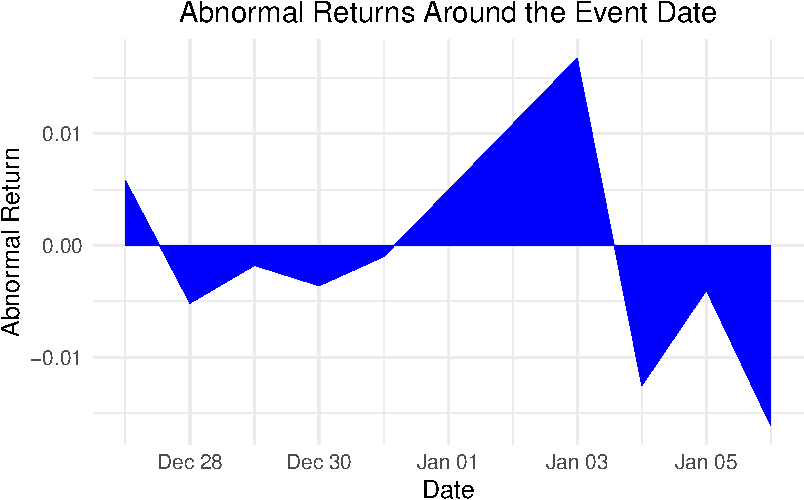
\includegraphics{CAR_files/figure-pdf/unnamed-chunk-8-1.pdf}

\section{Conclusion}\label{conclusion}

In this document, we extended the analysis from estimating the beta
coefficient to measuring cumulative abnormal returns (CAR). We estimated
the market model, calculated abnormal returns, and computed the CAR for
a specified event window. CAR is a useful measure in event studies to
assess the impact of specific events on a stock's price.



\end{document}
